\chapter{Mapping BPMN to Jiac AgentBeans}
\label{chap:mapping}
The element mapping from BPMN to Jiac AgentBeans is created based on the existing mapping to JiacV - JADL script. Compared to a JADL script, an AgentBean that is written completely in Java enables more possibilities in mapping concepts such as intermediate Event handling. Some concepts found in Wade's workflow implementation inspired us for the development of the mapping. This chapter will provide a detailed overview of the mapping.\\\\

%%%%%%%%%%%%%%%%%%%%%%%%%%%%%%%%%%%%%%%%%%%%%%%%%%%%%%%
% 4.1 Pools & Processes                               %
%%%%%%%%%%%%%%%%%%%%%%%%%%%%%%%%%%%%%%%%%%%%%%%%%%%%%%%
\section{Pools and Processes}
Every pool in a process diagram will be mapped into an AgentBean. The name of the AgentBean will be derived from the Pool name, and the name of the process diagram it is contained in. If a Pool with the same name (e.g Mathematican) is contained in the business process diagrams ExtractRoot and Faculty, then the two agent beans \texttt{Mathematican\_ExtractRoot} and \texttt{Mathematican\_Faculty} will be created. Further, they are grouped in the package mathematican. 

The process contained in a pool is mapped into a \textbf{workflow method}. Depending on the start event's type, this workflow method may be called in the execute method of the bean (for timer start event), it may be exposed as an action (for message start event with service implementation), or if the start event is a message start event with MessageChannel implementation, a SpaceObserver will be created and attached to the agent's memory, which will call the workflow method when a message with the payload and address as specified in the implementing message channel are written into the agent's memory.

The mapping of a task contained in a process flow will be wrapped in the so called \textbf{activity method} which will be called by the workflow method. Special cases for tasks with event handler and subprocesses will be discussed in a later section.

Lanes are currently ignored. A process of a lane will be handled as a process of the containing pool.

\begin{figure}[h]
	\centering
		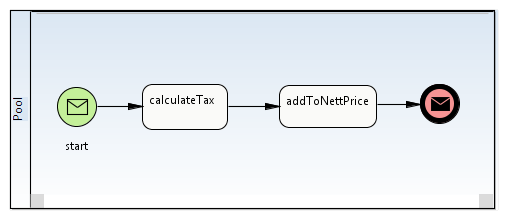
\includegraphics[width=0.80\textwidth]{images/mapping/pool_and_process.png}
	\caption{Mapping example : Pool and Process}
	\label{fig:pool+process}
\end{figure}

The Figure\ref{fig:pool+process} shows a simple example of a pool called Pool with the process doProcess. For the Pool, a Java class called Pool\_DoProcess will be created and it will have the workflow method called doProcess. In this example the message start event is implemented as a service, thus the workflow method is exposed as an Action as we can see in the following Listing \ref{list:pool+process}.  
\begin{lstlisting}[language = Java, caption =  Mapped element: Pool and Process (Figure \ref{fig:pool+process}), label = list:pool+process]
package pool;//derived from the pool name

//some imports...

public class Accounting_CalculatePrice extends AbstractMethodExposingBean{
	
	public final static String ACTION_DOPROCESS = "pool.Pool_DoProcess#doProcess"; 
	
	// process attribute would be declared here
	[...]
	@Expose(name = ACTION_DOPROCESS, scope = ActionScope.GLOBAL)
	public double doProcess(double nettPrice, double taxRateInPercent) {
		calculateTax();
		addToNettPrice();
		return totalPrice;
	}
	
	private void calculateTax(){
		[...]
	}
	
	private void addToNettPrice(){
		[...]
	}
}
\end{lstlisting}


\section{Workflow Structure}
Workflow structure is mapped as the content of the workflow method. It defines the invocation structure of the flow objects contained in a process.

\subsection{Sequence Flow}
The mapping of a sequence flow is trivial. The mapped elements connected with a sequence flow will be invoked sequentially in the workflow method (see Figure \ref{fig:mapping_sequence}).\\

\begin{figure}[h]
\begin{minipage}[c]{0.5\textwidth}
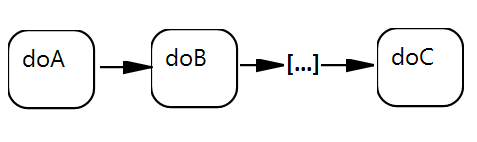
\includegraphics[width=0.9\textwidth]{images/mapping/sequence.png}
\end{minipage}
\begin{minipage}[c]{0.5\textwidth}
\begin{lstlisting}[language=Java]
doA();
doB();
[...]
doC();
\end{lstlisting}
\end{minipage}
\caption{Mapping Example: Sequence Flow}%
\label{fig:mapping_sequence}%
\end{figure}

\subsection{Gateways}
Branches of a gateway are wrapped according to the gateway's type. There are 5 different types of gateways:
\begin{enumerate}
	\item AND (Parallel)
	\item OR (Inclusive)
	\item XOR\_Data (Exclusive)
	\item XOR\_Event (Event Based)
	\item Complex 
\end{enumerate}

%%%%%%%%%%%%%%%%%%%%%%%%%%%%%%%%%%%
\textbf{AND-Gateway (Parallel)}\\
In an AND-Gateway, all branch will be wrapped in parallel to one another. At runtime all branches are executed within a thread. 
Figure \ref{fig:mapping_AND} shows an example of the mapping. \\

\begin{figure}[h]%
\begin{minipage}[c]{0.5\textwidth} 
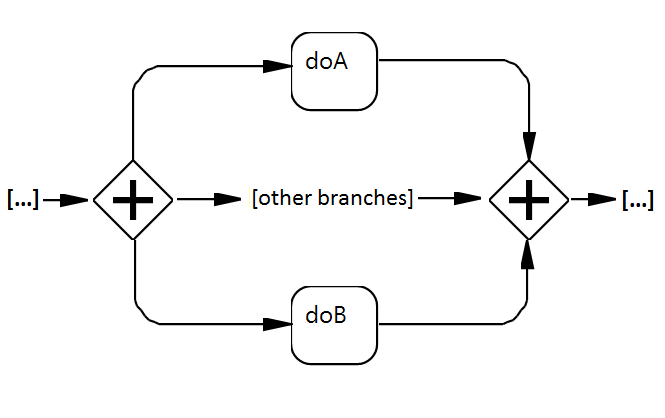
\includegraphics[width=0.95\linewidth]{images/mapping/and-gateway.png}
\end{minipage}
\begin{minipage}[c]{0.5\textwidth} 
\begin{lstlisting}[language=Java]
[...]
Thread and_branch1 = new Thread(){
	public void run(){
		doA();
	}
};
[create thread for other branches]
Thread and_branch2 = new Thread(){
	public void run(){
		doB();
	}
};
and_branch1.start();
[start other branches]
and_branch2.start();
try {
	and_branch1.join();
	[join other branches]
	and_branch2.join();
} catch(InterruptedException) { }
[...]
\end{lstlisting}
\end{minipage}
\caption{Mapping example: AND Gateway}%
\label{fig:mapping_AND}%
\end{figure}



%%%%%%%%%%%%%%%%%%%%%%%%%%%%%%%%%%%%%
\textbf{OR-Gateway (Inclusive)}\\
Branches of an OR-Gateway will also be executed in parallel to one another, but the content of a branch is additionally wrapped in an if-then block as shown in Figure \ref{fig:mapping_OR}. At runtime, the condition of each branches will be checked and the branch will be skipped if the condition does not hold. However, if the or-gateway has a branch with default condition, the default branch will only be executed if none of the other branches are executed.
\begin{figure}[h]
\begin{minipage}[c]{0.5\textwidth}
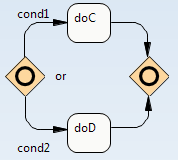
\includegraphics[width=0.95\textwidth]{images/mapping/or-gateway.png}
\end{minipage}
\begin{minipage}[c]{0.5\textwidth}
\begin{lstlisting}[language=Java]
[...]
Thread or_branch1 = new Thread(){
	public void run(){
		if(cond1){
			doA();
		}
	}
};
[thread for other branches]
Thread or_branch2 = new Thread(){
	public void run(){
		if(cond2){
			doB();
		}
	}
};
or_branch1.start();
[start other branches]
or_branch2.start();
try {
	or_branch1.join();
	[join other branches]
	or_branch2.join();
} catch(InterruptedException) { }
[...]
\end{lstlisting}
\end{minipage}
\caption{Mapping example: OR Gateway}%
\label{fig:mapping_OR}%
\end{figure}


\textbf{XOR\_Data-Gateway (Exclusive)}\\
Branches of an XOR\_Data are wrapped in an if-then-else block (see Figure \ref{fig:mapping_xorData}). Only one branch will actually be executed at runtime. \\

\begin{figure}[h]
\begin{minipage}[c]{0.5\textwidth}
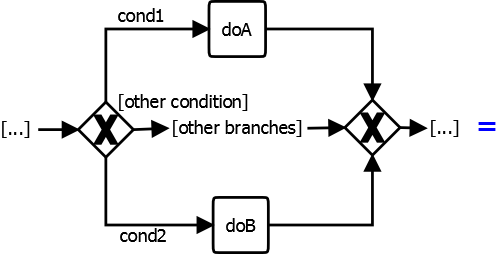
\includegraphics[width=0.95\textwidth]{images/mapping/xor-data.png}
\end{minipage}
\begin{minipage}[c]{0.5\textwidth}
\begin{lstlisting}[language=Java]
[...]
if(cond1){
	doA();
}else{
	if([other condition]){
		[other branches]
	}else{
		if(cond2){
			doB();
		}
	}
[...]
\end{lstlisting}
\end{minipage}
\caption{Mapping example: XOR\_Data Gateway}%
\label{fig:mapping_xorData}%
\end{figure}

\textbf{XOR\_Event-Gateway (Event Based)}\\
For XOR\_Event, a waiting loop will be started in a Thread, and an EventHandler (an extension to java.lang.Thread) instance for each branch will be created and started, according to the event's trigger of each branch. If an event handler receive an event, the waiting thread will be stopped, and the process continues with the elements of the branch, and other branches will be skipped. Figure \ref{fig:mapping_xorEvent} shows an example of the mapping.

\begin{figure}[h]
\begin{minipage}[c]{0.5\textwidth}
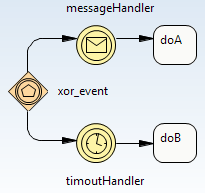
\includegraphics[width=0.9\textwidth]{images/mapping/xor-event.png}
\end{minipage}
\begin{minipage}[c]{0.5\textwidth}
\begin{lstlisting}[language=Java]
[...]
Thread xor_event_wait = new Thread(){
	public void run() {
		while(true) {
			try {
				Thread.sleep(100);
			} catch(InterruptedException e) {}
		}
	}
};
MessageEventHandler messageHandler = new MessageEventHandler(xor_event_wait);
[handler for other branches]
TimeoutEventHandler timeoutHandler = new TimeoutEventHandler(20000, xor_event_wait);
//start the wait activity and all handlers
xor_event_wait.start();
messageHandler.start();
[start other handlers]
timeoutHandler.start();
try{
	xor_event_wait.join();
	timeoutHandler.stop();
	[stop other handlers]
	messageHandler.stop();
} catch (InterruptedException e) {
	if(messageHandler.hasBeenTriggered()){
		doA();
	}
	[other branches]
	if(timeoutHandler.hasBeenTriggered()){
		doB();
	}
}
[...]
\end{lstlisting}
\end{minipage}
\caption{Mapping example: XOR\_Event Gateway}%
\label{fig:mapping_xorEvent}%
\end{figure}
\newpage
The event handler class will be added as an inner class to the bean, and they will have a constructor with a Thread toStop argument (among other arguments) and a boolean method \verb|hasBeenTrigerred()| to check whether the event handler has been activated by the expected event. The following Listing \ref{list:timeoutEventHandler} shows an implementation of the TimeoutEventHandler. This inner class will be included in every agent bean class that uses a TimeoutEventHandler.\\\\

\begin{lstlisting}[language=Java, caption=TimeoutEventHandler implementation as an inner class, label=list:timeoutEventHandler]
class TimeoutEventHandler extends Thread{
		
		long timeout;
		Thread toStop;
		boolean triggered = false;
		
		public TimeoutEventHandler(long timeout, Thread toStop){
			this.timeout = timeout;
			this.toStop = toStop;
		}
		
		public void run(){
			try {
				Thread.sleep(timeout);
				triggered = true;
				toStop.stop();
			}catch(InterruptedException e ) { }
		}
		
		public boolean hasBeenTriggered(){
			return triggered;
		}
		
}
\end{lstlisting}

\textbf{Complex-Gateway}\\
A mapping concept for Complex Gateways has not been developed in the current Version. \\

\subsection{Loop Blocks}
Structured loop blocks are mapped as shown in Figure \ref{fig:mapping_loop}.
\begin{figure}[h]
\begin{minipage}[c]{0.5\textwidth}
	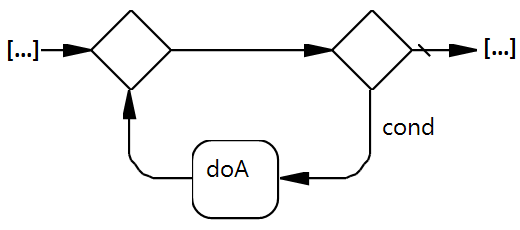
\includegraphics[width=0.95\textwidth]{images/mapping/loop_block.png}
\end{minipage}
\begin{minipage}[c]{0.5\textwidth}
\begin{lstlisting}[language=Java]
[...]

while(cond){
	doA();
}

[...]
\end{lstlisting}
\end{minipage}
\caption{Mapping example: Loop Blocks }%
\label{fig:mapping_loop}%
\end{figure}

While the condition applies, the content branch will be repeated. 

\begin{figure}[h]
\begin{minipage}[c]{0.45\textwidth}
	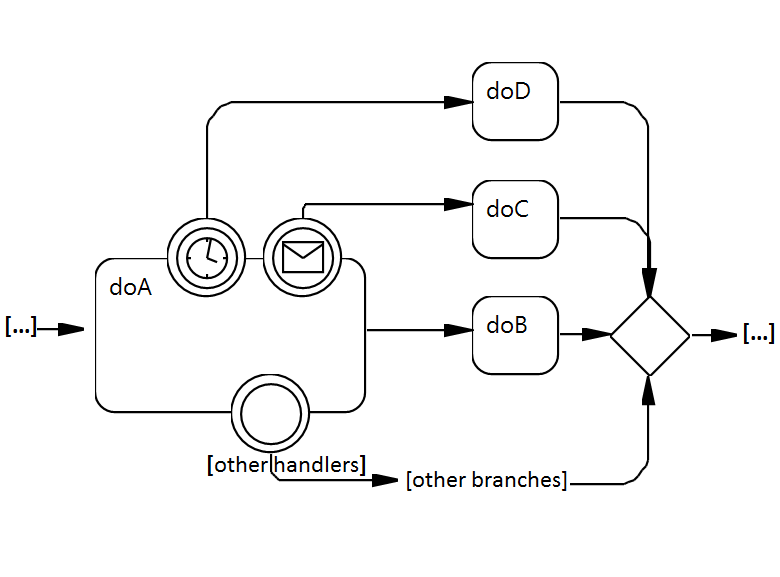
\includegraphics[width=0.95\textwidth]{images/mapping/event_handler.png}
\end{minipage}
\begin{minipage}[c]{0.55\textwidth}
\begin{lstlisting}[language=Java]
[...]
Thread doA_Thread = new Thread(){
	public void run(){
		doA();
	}
};
MessageEventHandler messageHandler = new MessageEventHandler(doA_Thread);
TimeoutEventHandler timeoutHandler = new TimeoutEventHandler(20000, doA_Thread);
[other handlers]

doA_Thread.start();
messageHandler.start();
timeoutHandler.start();
[start other handlers]

try{
	doA_Thread.join();
	timeoutHandler.stop();
	messageHandler.stop();
	[stop other handlers]
} catch(InterruptedException e) {
	if(messageHandler.hasBeenTriggered(){
		doC();
	}
	if(timeoutHandler.hasBeenTriggered(){
		doD();
	}
	if([other handlers].hasBeenTriggered()){
		[...]
	}
}

//doB only if none of the 
//event handlers are triggered
if(!messageHandler.hasBeenTriggered()){
	if(!timeoutHandler.hasBeenTriggered()){
		if(![other handlers].hasBeenTriggered()){	
			doB(); 
		}
	}
}

[...]
\end{lstlisting}
\end{minipage}
\caption{Mapping example: Event Handler}%
\label{fig:mapping_eventhandler}%
\end{figure}

\subsection{Event Handler}
As we can see in Figure \ref{fig:mapping_eventhandler}, the mapping of an Event Handler attached to an activity is somewhat similar to the mapping of gateway event. Instead of the waiting thread, a thread calling the activity method will be created, and it will be stopped if the event handler is triggered.\\

\newpage
\section{Activites}
Now we will discuss the activities in details. Activities are divided into tasks and subprocess. As mentioned before, a task will be wrapped in an activity method. This enables each task to have their own scope of properties. The properties of subprocesses however, should be shared with all activities contained in it. Therefore wrapping subprocesses in a method is not enough. Instead a subprocess will be wrapped in an inner class.
 
\subsection{Tasks}
Basically, the activity method generated from a task will look like what we can see in Figure \ref{fig:mapping_task}:

\begin{figure}[h]
\begin{minipage}[c]{0.3\textwidth}
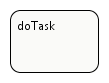
\includegraphics[width=0.95\textwidth]{images/mapping/task.png}
\end{minipage}
\begin{minipage}[c]{0.7\textwidth}
\begin{lstlisting}[language=Java]
public void doTask(){
	[declaration of properties]
	[start assignments]
	[special mapping depending on task-type]
	[end assignments]
}
\end{lstlisting}
\end{minipage}
\caption{Mapping example: Task}%
\label{fig:mapping_task}%
\end{figure}
\newpage
The method will start by declaring java variables, derived from the task's properties (if any exists). After the declaration, start assignments will take place, followed by the task's actual mapping (if any, depending on the task type). Finnaly, the code will be closed with the end assignments. The BPMN allows us to specify properties and assignments (including when the assignment should take place) in the task's property sheet. Thus, other than the workflow model in Wade, it is possible to generate the operations needed to execute the activity completely from the model. Now let's take a closer look on how specific task types are being mapped.\\

\textbf{Script-task}\\
For Script-tasks, the script defined in the task's property will be directly added into the activity-method. This type of task is comparable to Wade's \textit{Code Activity}, but just like the properties and assignments, with BPMN the script can be specified in the property sheet of the task. For the transformation to agent beans, the given script should be a valid Java expression. \\\\


\textbf{Service-task}\\
A service task is mapped into an invocation of an Action defined by other Bean.\\

\begin{figure}[h]
\begin{minipage}[c]{0.3\textwidth}
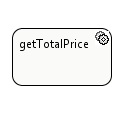
\includegraphics[width=0.95\textwidth]{images/mapping/service_task.png}
\end{minipage}
\begin{minipage}[c]{0.7\textwidth}
\begin{lstlisting}[language=Java]
[...]
Action [operation] = retrieveAction([interface].[operation]);
Serializeable [] results = invokeAndWaitForResults([operation], new Serializeable[]{[inputs]}).getResults();
[assign outputs from results]
[...]
\end{lstlisting}
\end{minipage}
\caption{Mapping example: Service-task}%
\label{fig:service_task}%
\end{figure}
Figure \ref{fig:service_task} shows how a service task would be mapped. First, the action has to be found. Then the service will be invoked and the result will be assign to the outputs defined in the task's implementing Service.\\\\

\textbf{Send-task}\\
A Send task will be mapped into an invocation of the ICommunicationBean's send action (see Figure \ref{fig:send_task}). The group address, to which the message should be sent, and the message itself will be derived from the given MessageChannel in the task's properties. \\\\
 
\begin{figure}[h]
\begin{minipage}[c]{0.3\textwidth}
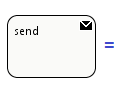
\includegraphics[width=0.95\textwidth]{images/mapping/sendTask.png}
\end{minipage}
\begin{minipage}[c]{0.7\textwidth}
\begin{lstlisting}[language=Java]
[...]
Action sendAction = retrieveAction(ICommunicationBean.ACTION_SEND);
IGroupAddress groupAddress = CommunicationAddressFactory.createGroupAddress([address]);
JiacMessage jiacMessage = new JiacMessage([payload]);
invoke(sendAction, new Serializable[]{jiacMessage, groupAddress});
[...]
\end{lstlisting}
\end{minipage}
\caption{Mapping example: Send-task}%
\label{fig:send_task}%
\end{figure}


\textbf{receive-task}\\
A receive-task will be mapped into a Java-Code that reads the memory and wait until the specified message defined by the given MessageChannel is found in the memory. \\

\begin{figure}[h]
\begin{minipage}[c]{0.3\textwidth}
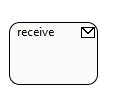
\includegraphics[width=0.95\textwidth]{images/mapping/receiveTask.png}
\end{minipage}
\begin{minipage}[c]{0.7\textwidth}
\begin{lstlisting}[language=Java]
[...]
Action joinAction = retrieveAction(ICommunicationBean.ACTION_JOIN_GROUP);
Action leaveAction = retrieveAction(ICommunicationBean.ACTION_LEAVE_GROUP);
IGroupAddress groupAddress = CommunicationAddressFactory.createGroupAddress([address]);
invoke(joinAction,new Serializable[]{groupAddress});
[payload] = null;
while([payload name]==null) {
	Set<IFact> all = memory.readAll();
	for(IFact fact : all){
		if(fact instanceof JiacMessage) {
			JiacMessage jiacMessage = (JiacMessage)fact;
			if(jiacMessage.getPayload() instanceof Ping && jiacMessage.getHeader(IJiacMessage.Header.SEND_TO).equals(groupAddress)) {
				memory.remove(jiacMessage);
				[payload name] = ([payload type]) jiacMessage.getPayload();
				break;
			}
		}
	}
	try{
		Thread.sleep(100);
	} catch(InterruptedException e) { }
}
invoke(leaveAction, new Serializable[]{groupAddress});
[...]
\end{lstlisting}
\end{minipage}
\caption{Mapping example: receive-task}%
\label{fig:receive_task}%
\end{figure}

\textbf{Call-task}\\
A call task will be mapped to an invocation of the called element. If the called element is an activity, then the activity method will be called. 
If the called element is a Pool, then the call task will be mapped into a service invocation. 

\textbf{User task}\\
The mapping of user tasks has not been completely developed yet. User tasks requires a User Interface module to get inputs from the user. To make it simple we can put a TODO flag in the code, and the developer should implement the UI manually. 

\textbf{Manual task}\\
Manual tasks won't be executed manually, therefore a mapping won't be needed.

\textbf{BusinessRule-tasks}\\
The mapping of business rule tasks doesn't exist in this Version.

\subsection{Subprocess}
A subprocess will be mapped into an inner class of the containing Process or Subprocess. This way it's properties can be shared among all tasks contained in it. The inner subprocess will have the method \texttt{public void run()} containing the workflow (similar to the bean's workflow method). The following example shows the mapping of a subprocess:\\

\begin{figure}[h]
\begin{minipage}[c]{0.3\textwidth}
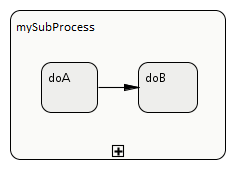
\includegraphics[width=0.95\textwidth]{images/mapping/subprocess.png}
\end{minipage}
\begin{minipage}[c]{0.7\textwidth}
\begin{lstlisting}[language=Java]
//workflow-method
public void doProcess{
[...]
MySubProcess mySubProcess = new MySubProcess();
mysubProcess.run();
[...]
}

[...]
// subprocess as Innerclass
class MySubProcess {
	[declaration of properties]
		
	public void run(){
		doA();
		doB();
	}
	
	private void doA(){
		[...] 
	}
	
	private void doB(){ 
		[...] 
	}
}
\end{lstlisting}
\end{minipage}
\caption{Mapping example : Subprocess}%
\label{fig:mapping_subprocess}%
\end{figure}

\subsection{Activity-Looping}
An activity can have a looping property. This will result in the wrapping of the task-specific mapping in a while-block. 
There are two types of activity-looping in BPMN:
\begin{enumerate}
	\item Standard-Loop
	\item Multi Instance Loop
\end{enumerate}
While the mapping of a standard-loop is trivial, the semantics of the multi instance loop is not very clear. Thus, a mapping of multi instance loop is not yet included in this version.
 
\textbf{Standard-Loop}
In a standard loop, the task specific mapping will be wrapped in a while block. The other elements of the activity method (variable declarations and assignments) will not be wrapped.  In Figure \ref{fig:mapping_standardLoop} we can see an example of a script task with a standard loop.
\begin{figure}[h]
\begin{minipage}[c]{0.3\textwidth}
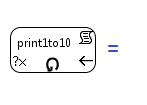
\includegraphics[width=0.95\textwidth]{images/mapping/standard_loop.png}
\end{minipage}
\begin{minipage}[c]{0.7\textwidth}
\begin{lstlisting}[language=Java]
public void print1To10(){
	int index;
	[more variable declarations]
	index= 1;
	[more start assignments]
	while((index < 11)) {
		System.out.println(index++);
	}
	[end assignments]
}
\end{lstlisting}
\end{minipage}
\caption{Mapping example : Activity-Looping (Standard Loop)}% 
\label{fig:mapping_standardLoop}%
\end{figure}

\section{Events}
Finally, we will now discuss the mapping of BPMN Events to Jiac AgentBeans. We will first discuss the Intermediate events and then we will handle Start and End Events. We need to group start and end events because the mapping will have influence on how the process will be started, and they will also determine the signature (input and output parameters) of the workflow method. 

\subsection{Intermediate-Events}
Intermediate Events are something that happens during the process. It's mapping will be added into the workflow method. To keep the workflow method readable, we decided to wrap intermediate events in a method (similar to activities). The name will be derived from the events name (if specified) or id, added with an event-type specific postfix.

In this version only the mapping of Timer and Message intermediate events are included. 

\textbf{Timer}\\
A timer intermediate event will turn the process to sleep until the given time expression. If the given time expression is a duration (option as duration in the property sheet is selected), then the expression will be handled as a long integer that defines how long (in milliseconds) the process should be paused.\\

If the given time is an exact time (e.g. Friday, November 4th 2011 10:00:00), then the expression should be parsed into a Java Date object and the process should be paused until the given date. However, it is not clear yet on how to handle incomplete date expressions (e.g. when we need to start a process every day at midnight). At the moment, the given date expression has to be in the form ''yyyy-MM-dd'T'HH:mm:ss.SSSZ'' (e.g. 2011-11-04T10:00:00.000+0100 for Friday, November 4th 2011 10:00:00). Figure \ref{fig:timer_intermediate}
shows an example of the mapping for both variants.
\begin{figure}[h]
\begin{minipage}[c]{0.28\textwidth}
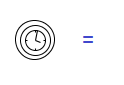
\includegraphics{images/mapping/timer_intermediate.png}
\end{minipage}
\begin{minipage}[c]{0.72\textwidth}
If the expression is a duration:
\begin{lstlisting}[language = Java]
[...]
try {
	Thread.sleep([time expression]);
} catch(InterruptedException e) {
}
[...]
\end{lstlisting}
If the expression is an exact time:
\begin{lstlisting}[language = Java]
[...]
try {
Date then = new SimpleDateFormat("yyyy-MM-dd'T'HH:mm:ss.SSSZ").parse([time expression]);
long toSleep = then.getTime() - System.currentTimeMillis();
if(toSleep>0){
	try {
		Thread.sleep(toSleep);
	} catch(InterruptedException e) {
	}
}
} catch(ParseException e) {
	System.out.println("ParseException: Time has to be in yyyy-MM-dd'T'HH:mm:ss.SSSZ form");
	e.printStackTrace();
}
[...]
\end{lstlisting}
\end{minipage}
\caption{Mapping example : Timer Intermediate Event}%
\label{fig:timer_intermediate}%
\end{figure}
\newpage
\textbf{Message}\\
Message intermediate events will be mapped similarly to a receive task. The process read the memory and wait until the expected message is found in the memory. 

\subsection{Start and End Events}

\textbf{Timer}\\
If a process starts with a timer event, then the workflow method will be called in the execute method. If the given time expression is a duration, the process will be started periodically. If the given time is an exact date, then the date will be parsed, and the process will be started when the date is passed. Figure \ref{fig:timer_start} shows an example of the mapping for both variants.

\begin{figure}[h]
\begin{minipage}[c]{0.28\textwidth}
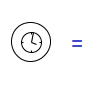
\includegraphics{images/mapping/timer_start.png}
\end{minipage}
\begin{minipage}[c]{0.72\textwidth}
If the expression is a duration:
\begin{lstlisting}[language = Java]
public void execute(){
	while(true){
		[start process]
		try {
			Thread.sleep([time expression]);
		} catch(InterruptedException e) {
		}
	}
}
\end{lstlisting}
If the expression is an exact time:
\begin{lstlisting}[language = Java]
public void execute(){
	try {
			Date then = new SimpleDateFormat("yyyy-MM-dd'T'HH:mm:ss.SSSZ").parse("2011-11-04T10:00:00.000+0100");
			long toSleep = then.getTime() - System.currentTimeMillis();
			if(toSleep>=0){
				try {
					Thread.sleep(toSleep);
				} catch(InterruptedException e) {
				}
				[start process]
			}
		} catch(ParseException e) {
			System.out.println("ParseException: Time has to be in yyyy-MM-dd'T'HH:mm:ss.SSSZ form");
			e.printStackTrace();
		}
}
\end{lstlisting}
\end{minipage}
\caption{Mapping example : Timer Start Event}%
\label{fig:timer_start}%
\end{figure}
\newpage

\textbf{Message}\\
Message Start and End events will influence the signature of the workflow method. The start event defines the parameters and the end event defines it's return type. We can divide message start and end events according to the event's implementation (Service or MessageChannel). 

\textbf{Message with Service implementation}
If the implementation is a Service, the workflow method will be exposed as an action(service). The process will be started by other AgentBean as a service by invoking the exposed action. The signature of the workflow method will be derived from the signature of the implementing service. 
Multiple return type are wrapped in a Serializable array. 

In Figure \ref{fig:message_service} we can see an example mapping of message start and end events with service implementation. The generated workflow method are exposed as an Action with the @Expose code in Line 5. 
\begin{figure}[h]
\begin{minipage}[c]{0.35\textwidth}
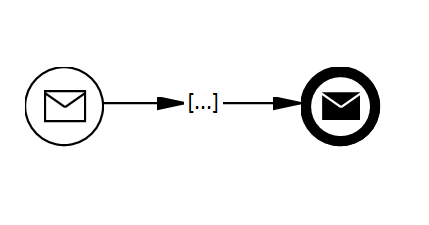
\includegraphics[width=0.9\textwidth]{images/mapping/messageStart.png}
\end{minipage}
\begin{minipage}[c]{0.65\textwidth}
\begin{lstlisting}[language = Java]
public class [Bean-name] extends AbstractMethodExposingBean{
	public final static String ACTION_[workflow name] = "[bean fullname]#[workflow method]"; 
	[...]
	
	@Expose(name = ACTION_[workflow name], scope = ActionScope.GLOBAL)
	public [service output] [workflow method]([service inputs]){
		[...]
		return [service output];
	}
	
	[...]
}
\end{lstlisting}
\end{minipage}
\caption{Mapping example : Message Start and End Events with Service Implementation}%
\label{fig:message_service}
\end{figure}


\newpage
\textbf{Message with MessageChannel implementation}\\
If the implementation is a MessageChannel, an observer will be created and attached to the agent's memory in the \verb|doStart()| method.
The workflow method will get the MessageChannel's payload as a parameter, and it will have no return type (void) and the result will be sent as a message to the specified MessageChannel of the end event. Figure \ref{fig:channel_start} shows a mapping example of a message start event, and in Figure \ref{fig:channel_end}, we can see a mapping example of how a message end event will be mapped.
\begin{figure}[h]
\begin{minipage}[c]{0.28\textwidth}
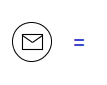
\includegraphics{images/mapping/message_start.png}
\end{minipage}
\begin{minipage}[c]{0.72\textwidth}
\begin{lstlisting}[language = Java]
public class [Bean-name] extends AbstractMethodExposingBean{
	[...]
	
	public void doStart(){
		[...]
		Action joinAction = retrieveAction(ICommunicationBean.ACTION_JOIN_GROUP);
		IGroupAddress groupAddress = CommunicationAddressFactory.createGroupAddress([channel]);
		invoke(joinAction,new Serializable[]{groupAddress});
		SpaceObserver<IFact> [event name or id]_observer = new SpaceObserver<IFact>(){
			public void notify(SpaceEvent<? extends IFact> event) { 
				if(event instanceof WriteCallEvent<?>){ 
					WriteCallEvent<IJiacMessage> wce = (WriteCallEvent<IJiacMessage>) event;
					IJiacMessage message = wce.getObject();
					IFact payload = message.getPayload();
					if(payload!=null && [payload name] instanceof [payload type]&& message.getHeader(IJiacMessage.Header.SEND_TO).equals([channel]){
						memory.remove(message);
						[workflow method](([payload type])payload);
					}
				}
			}
		};
		memory.attach(_nO3bwPwdEeCOWB3dJOsUA_observer);
		[...]
	}
	
	public void [workflow method]([payload type] [payload name]){
		[...]
	}
	
	[...]
}
\end{lstlisting}
\end{minipage}
\caption{Mapping example : Message Start Event with MessageChannel Implementation}%
\label{fig:channel_start}
\end{figure}


\begin{figure}[hbtp]
\begin{minipage}[c]{0.28\textwidth}

\includegraphics{images/mapping/message_end.png}
\end{minipage}
\begin{minipage}[c]{0.72\textwidth}
\begin{lstlisting}[language = Java]
public class [Bean-name] extends AbstractMethodExposingBean{
	[...]
	public void [workflow method]([payload type] [payload name]){
		[...]
		[payload type] [payload name]//payload variable declaration
		[payload name]= new StringOutput("ok");//payload assignment
		Action sendAction = retrieveAction(ICommunicationBean.ACTION_SEND);
		IGroupAddress groupAddress = CommunicationAddressFactory.createGroupAddress([channel]);
		JiacMessage jiacMessage = new JiacMessage([payload name]);
		invoke(sendAction, new Serializable[]{jiacMessage, groupAddress});
	}
	[...]
}
\end{lstlisting}
\end{minipage}
\caption{Mapping example : Message End Event with MessageChannel Implementation}%
\label{fig:channel_end}
\end{figure}
\newpage
\section{Open Issues}

In this chapter, we presented the details of the mapping from BPMN to Jiac AgentBeans. As we can see in some sections, there are some elements that has not been mapped yet. In the future, we will need to study the semantics of the unmapped elements (e.g. multi instance loop, rule events etc.) further and develop their mapping.